\scanpage{101}
\[
\left\{\begin{aligned}
 X&=\mathbb{P}^{2}-T'\\
 Y&=T-T'\\
 U&=\mathbb{P}^{2}-T
\end{aligned}\right.
\]

\figure{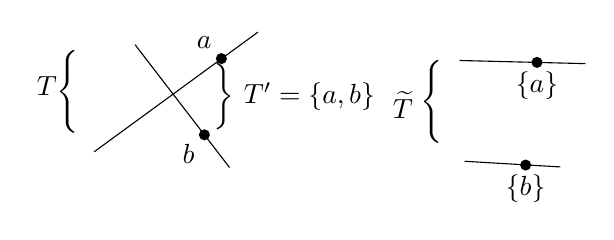
\begin{tikzpicture}[x=.8cm,y=.8cm]
\node at (-.75,1.05) {$T$};
\node at (-.42,.95) {$\Biggl\{$};
\draw (0,0)--(2.6,1.9);
\draw (.65,1.7)--(2.15,-.25);
\fill (2.02,1.48) circle (2pt) node[above left] {$a$};
\fill (1.75,.27) circle (2pt) node[below left] {$b$};
\node at (2.06,.87) {$\biggr\}$};
\node[right] at (2.22,.87) {$T'=\{a,b\}$};
\node at (4.9,.75) {$\widetilde T$};
\node at (5.35,.8) {$\Biggl\{$};
\draw (5.8,1.45)--(7.8,1.40);
\draw (5.88,-.15)--(7.4,-.24);
\fill (7.03,1.42) circle (2pt) node[below] {$\{a\}$};
\fill (6.85,-.21) circle (2pt) node[below] {$\{b\}$};
\end{tikzpicture}}

\diagram{\begin{tikzcd}[ampersand replacement=\&,column sep=small]
H^1(\widetilde Y)\deleted{\unsure{\leftarrow|=}}\arrow[dr] \& \& \\
H^3_Y(X)\arrow[r] \& H^{3}_{\deleted{\unsure{!|Y}}}(X)\arrow[r,dash] \& H^3(U)
\end{tikzcd}}

\diagram{\begin{tikzcd}[ampersand replacement=\&,column sep=small]
H^1_!(Y) \& H^1_!(X)\arrow[l]\arrow[dl] \& H^1_!(U)\arrow[l] \& H^0(\\
H^1_!(\widetilde Y) \& \& {\substack{\Vert\\0\ \text{car }T\ \text{connexe}}}
\end{tikzcd}}

\diagram{\begin{tikzcd}[ampersand replacement=\&,column sep=small,row sep=small]
H^0(\widetilde T')\arrow[r] \& H^0_{\unsure{!|1|{}}}(\widetilde T)\arrow[r] \& H^1_!(\widetilde Y)\arrow[r] \& H^1(\widetilde T')\\
H^0(\mathbb P^2)\arrow[r]\arrow[u] \& H^0_{\unsure{!|{}}}(T')\arrow[r]\arrow[u] \& H^1_!(X)\arrow[r]\arrow[u] \& {\underset{\substack{\Vert\\\unsure{0|1|{}}}}{H^1(\mathbb P^2)}}\arrow[u]\\
H^0(P^2)\arrow[r] \& H^0(T)\arrow[r]\arrow[u] \& H^1_!(U)\arrow[r]\arrow[u] \& {\underset{\substack{\Vert\\\unsure{0|1|{}}}}{H^1(P^2)}}
\end{tikzcd}}

\margin{$\left\{\begin{aligned}&T\ \text{\uline{connexe}}\\ &T'\ \text{disconnexe, \deleted{et}}\end{aligned}\right.$ contenu \unsure{ds|dans} \unsure{lieu|lieux}. \deleted{\unsure{lieu}} de lissité, et tte comp. de $T'$ contient au plus un point de $T'$.}

\diagram{\begin{tikzcd}[ampersand replacement=\&,column sep=tiny,row sep=large]
\& \& H^0(T')/\operatorname{Im}H^0(\mathbb P^2)\arrow[dl,"{\text{\unsure{inj|isog|isom} ?}}"] \& {\underset{\substack{\Vert\\0}}{H^0(T)/\operatorname{Im} H^0(\mathbb P^2)}}\arrow[l]\\
H^1_!(\widetilde Y)\ \unsure{\supset|\rightarrow} \& {H^0(\widetilde T/\operatorname{Im}H^0(\widetilde T')\,{}_{\ =0}} \& \&
\end{tikzcd}}

\[
\deleted{\unsure{H^1_!|H^1_4}}
\]
\noindent\rule{\linewidth}{0.4pt}
% archive sheet number: 100
